\documentclass[11pt,a4paper]{report}

% ---------- Packages ----------
\usepackage[utf8]{inputenc}
\usepackage[T1]{fontenc}
\usepackage[french]{babel}
\usepackage{lmodern}
\usepackage{geometry}
\geometry{margin=2.4cm}

\usepackage{amsmath,amssymb,amsthm}
\usepackage{graphicx}
\usepackage{xcolor}
\usepackage{tikz}
\usetikzlibrary{arrows.meta, positioning, fit, backgrounds}
\usepackage{booktabs}
\usepackage{enumitem}
\usepackage{hyperref}
\usepackage{listings}
\usepackage{caption}
\usepackage{subcaption}
\usepackage{fancyhdr}
\usepackage{tcolorbox}
\tcbuselibrary{skins,breakable}

\hypersetup{
    colorlinks=true,
    linkcolor=blue!50!black,
    citecolor=blue!50!black,
    urlcolor=blue!50!black,
    pdftitle={Text-to-Image : Diffusion et Flow Matching},
    pdfauthor={Felix Bos},
}

\definecolor{codebg}{RGB}{245,245,248}
\lstset{
    backgroundcolor=\color{codebg},
    basicstyle=\ttfamily\footnotesize,
    breaklines=true,
    frame=single,
    rulecolor=\color{gray!40},
    columns=fullflexible,
    keywordstyle=\color{blue!60!black}\bfseries,
    commentstyle=\color{green!40!black},
    stringstyle=\color{orange!60!black},
    showstringspaces=false,
}

% Boîte "intuition" utilisée dans tout le document.
\newtcolorbox{intuition}[1][]{
    enhanced, breakable, colback=blue!4, colframe=blue!40!black,
    fonttitle=\bfseries, title=Intuition, #1
}
\newtcolorbox{remarque}[1][]{
    enhanced, breakable, colback=yellow!8, colframe=orange!60!black,
    fonttitle=\bfseries, title=Remarque, #1
}
\newtcolorbox{codebox}[1][]{
    enhanced, breakable, colback=gray!4, colframe=gray!50!black,
    fonttitle=\bfseries\ttfamily, #1
}

\newtheorem{definition}{Définition}[chapter]
\newtheorem{propriete}{Propriété}[chapter]

\setlength{\headheight}{14.5pt}
\renewcommand{\chaptermark}[1]{\markboth{\thechapter.\ #1}{}}
\pagestyle{fancy}
\fancyhf{}
\fancyhead[L]{\small\leftmark}
\fancyhead[R]{\small\itshape Diffusion \& Flow Matching}
\fancyfoot[C]{\thepage}
\renewcommand{\headrulewidth}{0.4pt}

\title{
    \Huge\textbf{Génération d'images à partir de texte} \\[0.3cm]
    \Large Modèles de diffusion et Flow Matching, de la théorie à l'implémentation \\[0.5cm]
    \large Un cours accompagné d'une implémentation complète en PyTorch
}
\author{Felix Bos}
\date{\today}

\begin{document}

\maketitle

\tableofcontents

\chapter*{Avant-propos}
\addcontentsline{toc}{chapter}{Avant-propos}

Ce document a deux objectifs.

Le premier est pédagogique : présenter, de manière aussi intuitive que rigoureuse, les deux grandes
familles de modèles génératifs par transport continu de distribution qui dominent aujourd'hui la
génération d'images — les \textbf{modèles de diffusion} (DDPM) et le \textbf{Flow Matching} — en
partant des bases (qu'est-ce qu'un modèle génératif, pourquoi la génération d'images est un problème
difficile) jusqu'aux détails d'implémentation (architecture U-Net, conditionnement par texte,
classifier-free guidance).

Le second objectif est documentaire : ce cours sert de référence théorique au dépôt de code qui
l'accompagne (\texttt{text-\linebreak[1]to-\linebreak[1]image-\linebreak[1]generative-\linebreak[1]models}),
une implémentation \emph{from scratch} en PyTorch des deux approches, entraînée sur le jeu de données
CelebA-Dialog (visages annotés de légendes en langage
naturel), conçue pour tourner entièrement en local sur un Mac Apple Silicon (accélération MPS). Le
chapitre~\ref{chap:project} fait explicitement le lien entre chaque brique théorique et le fichier de
code qui l'implémente.

\begin{intuition}
Le fil conducteur de tout ce document tient en une phrase : \textbf{un modèle génératif de ce type
n'apprend pas à dessiner une image directement} — il apprend une règle de transformation simple
(« comment transformer un peu de bruit en quelque chose d'un peu plus net ») et on obtient une image
en appliquant cette règle un grand nombre de fois. La diffusion et le flow matching ne diffèrent que
par la nature de cette règle et la façon dont on l'apprend.
\end{intuition}

\paragraph{Comment lire ce document.} Les chapitres~\ref{chap:generative} à~\ref{chap:architecture}
constituent le cours proprement dit et sont indépendants du projet : ils se lisent comme une
introduction générale aux modèles de diffusion et de flow matching. Le chapitre~\ref{chap:project} est
spécifique à l'implémentation et suppose les chapitres précédents acquis.

\chapter{Modèles génératifs : contexte et enjeux}
\label{chap:generative}

\section{Le problème de la génération}

On dispose d'un jeu de données $\{x^{(1)}, \dots, x^{(N)}\}$ — par exemple $N$ photographies de
visages — que l'on suppose échantillonnées indépendamment d'une distribution inconnue $p_{\text{data}}$
sur un espace de très grande dimension (une image $64\times 64$ en couleur vit dans
$\mathbb{R}^{64 \times 64 \times 3} = \mathbb{R}^{12288}$).

\begin{definition}[Modèle génératif]
Un modèle génératif est une procédure qui, sans connaître $p_{\text{data}}$ explicitement, permet de
produire de nouveaux échantillons $x \sim p_\theta$ où $p_\theta$ est une distribution apprise à
partir des données, censée approcher $p_{\text{data}}$.
\end{definition}

La difficulté centrale n'est pas de mémoriser les données d'entraînement (un modèle qui recopie une
image du jeu d'entraînement au hasard \og génère \fg\ techniquement une image plausible, mais n'a rien
appris d'utile) : elle est de capturer la \emph{structure} de $p_{\text{data}}$ suffisamment bien pour
produire des échantillons \textbf{nouveaux} et \textbf{plausibles}. Pour des visages, cela veut dire
respecter implicitement des milliers de contraintes non écrites (deux yeux symétriques, une peau dont
la texture est cohérente avec l'éclairage, des proportions anatomiquement crédibles) sans qu'aucune de
ces contraintes n'ait été programmée à la main.

\section{Un bref panorama des approches}

\subsection{Modèles à variable latente explicite : les VAE}

Un \emph{auto-encodeur variationnel} (VAE) apprend conjointement un encodeur $q_\phi(z \mid x)$, qui
compresse une image $x$ en un vecteur latent $z$ de basse dimension, et un décodeur $p_\theta(x \mid z)$,
qui reconstruit une image à partir de $z$. En imposant que $z$ suive approximativement une loi normale
$\mathcal{N}(0, I)$, on peut, après entraînement, générer une nouvelle image en tirant
$z \sim \mathcal{N}(0, I)$ et en appliquant le décodeur.

\begin{intuition}
Le VAE apprend une \og carte \fg\ compacte de l'espace des images : chaque point de cette carte (le
latent $z$) correspond à une image. Générer, c'est piocher un point au hasard sur la carte.
\end{intuition}

En pratique, les VAE produisent des images souvent légèrement floues : la loss (une borne inférieure
de la vraisemblance, l'ELBO) pénalise moins une image \og moyennée \fg\ qu'une hallucination nette
mais incorrecte, ce qui pousse le modèle vers des reconstructions prudentes.

\subsection{Modèles adversariaux : les GAN}

Un \emph{Generative Adversarial Network} (GAN) oppose deux réseaux : un générateur $G$ qui transforme
du bruit en image, et un discriminateur $D$ qui essaie de distinguer les vraies images des images
générées. Les deux réseaux s'entraînent simultanément, en compétition — le générateur cherchant à
tromper le discriminateur, le discriminateur cherchant à ne pas se laisser tromper.

Les GAN produisent typiquement des images très nettes (pas de flou caractéristique du VAE), mais
l'entraînement est notoirement instable (risque d'effondrement de mode, où le générateur cesse de
produire une variété d'images et se contente de reproduire quelques exemples qui trompent bien le
discriminateur) et ne dispose d'aucune fonction de perte directement interprétable pour suivre la
progression.

\subsection{Modèles à transport continu : diffusion et flow matching}

La famille qui nous intéresse dans ce document adopte une stratégie différente : au lieu d'apprendre
directement une transformation \og bruit $\to$ image \fg\ en une seule étape (comme le générateur d'un
GAN), on apprend une transformation \textbf{progressive}, décomposée en de nombreux petits pas, chacun
faisant passer d'un état légèrement plus bruité à un état légèrement moins bruité (ou l'inverse selon
le sens dans lequel on parcourt le processus).

\begin{intuition}
Sculpter un bloc de marbre en une statue en un seul geste est presque impossible. Le faire par des
milliers de petits coups de burin successifs, chacun corrigeant légèrement la forme précédente, est
beaucoup plus faisable — même si aucun coup de burin individuel ne \og sait \fg\ à quoi ressemblera la
statue finale. C'est l'intuition centrale des modèles de diffusion et de flow matching : remplacer un
problème de génération difficile (un grand saut) par une séquence de problèmes de \emph{raffinement
local} beaucoup plus faciles (de petits pas).
\end{intuition}

Les deux chapitres suivants détaillent chacune de ces deux approches : les modèles de diffusion
(chapitre~\ref{chap:ddpm}), historiquement les premiers à obtenir des résultats compétitifs avec les
GAN sur la génération d'images, puis le flow matching (chapitre~\ref{chap:flow}), une formulation plus
récente et plus directe du même principe.

\begin{table}[h]
\centering
\begin{tabular}{@{}lccc@{}}
\toprule
& \textbf{VAE} & \textbf{GAN} & \textbf{Diffusion / Flow Matching} \\
\midrule
Entraînement & stable & instable & stable \\
Netteté des images & moyenne (flou) & élevée & élevée \\
Diversité des échantillons & bonne & risque d'effondrement & bonne \\
Coût de génération & 1 passe & 1 passe & de dizaines à milliers de passes \\
Loss interprétable & oui (ELBO) & non (jeu à somme nulle) & oui (MSE) \\
\bottomrule
\end{tabular}
\caption{Comparaison schématique des grandes familles de modèles génératifs d'images.}
\end{table}

Le prix à payer pour la stabilité d'entraînement et la qualité des modèles à transport continu est le
\textbf{coût de génération} : produire une seule image nécessite d'appeler le réseau de neurones de
nombreuses fois (typiquement de quelques dizaines à un millier de fois), contre une seule passe pour un
GAN ou un VAE. C'est un compromis assumé par toute cette famille de modèles, diffusion comme flow
matching.

\chapter{Les modèles de diffusion (DDPM)}
\label{chap:ddpm}

Ce chapitre présente les \emph{Denoising Diffusion Probabilistic Models} (DDPM), introduits par
Sohl-Dickstein et al. (2015) et popularisés par Ho, Jain et Abbeel (2020) \cite{ho2020ddpm}, qui sont
à l'origine de la vague de modèles text-to-image (DALL-E~2, Imagen, Stable Diffusion).

\section{Vue d'ensemble : deux processus}

Un DDPM est défini par deux processus, tous deux des chaînes de Markov à $T$ étapes ($T \approx 1000$
en pratique) :

\begin{itemize}
    \item le \textbf{processus direct} (\emph{forward process}), noté $q$, qui bruite progressivement
    une image $x_0$ jusqu'à obtenir un bruit gaussien pur $x_T$. Ce processus est \textbf{fixé}, sans
    paramètre à apprendre ;
    \item le \textbf{processus inverse} (\emph{reverse process}), noté $p_\theta$, qui tente de défaire
    ce bruitage pas à pas. C'est ce processus, paramétré par un réseau de neurones de poids $\theta$,
    que l'on entraîne.
\end{itemize}

\begin{center}
\begin{tikzpicture}[font=\small, node distance=2.1cm]
\node (x0) {$x_0$};
\node (x1) [right=of x0] {$x_1$};
\node (dots1) [right=of x1] {$\cdots$};
\node (xt) [right=of dots1] {$x_{t-1}$};
\node (xt1) [right=of xt] {$x_t$};
\node (dots2) [right=of xt1] {$\cdots$};
\node (xT) [right=of dots2] {$x_T$};

\draw[-Stealth, bend left=25, blue!60!black] (x0) to node[above]{$q(x_1|x_0)$} (x1);
\draw[-Stealth, bend left=25, blue!60!black] (x1) to node[above]{$q$} (dots1);
\draw[-Stealth, bend left=25, blue!60!black] (dots1) to node[above]{$q$} (xt);
\draw[-Stealth, bend left=25, blue!60!black] (xt) to node[above]{$q(x_t|x_{t-1})$} (xt1);
\draw[-Stealth, bend left=25, blue!60!black] (xt1) to node[above]{$q$} (dots2);
\draw[-Stealth, bend left=25, blue!60!black] (dots2) to node[above]{$q$} (xT);

\draw[-Stealth, bend left=25, red!70!black] (x1) to node[below]{$p_\theta(x_0|x_1)$} (x0);
\draw[-Stealth, bend left=25, red!70!black] (dots1) to node[below]{$p_\theta$} (x1);
\draw[-Stealth, bend left=25, red!70!black] (xt) to node[below]{$p_\theta$} (dots1);
\draw[-Stealth, bend left=25, red!70!black] (xt1) to node[below]{$p_\theta(x_{t-1}|x_t)$} (xt);
\draw[-Stealth, bend left=25, red!70!black] (dots2) to node[below]{$p_\theta$} (xt1);
\draw[-Stealth, bend left=25, red!70!black] (xT) to node[below]{$p_\theta$} (dots2);
\end{tikzpicture}
\end{center}

\begin{center}
{\color{blue!60!black}\textbf{Forward} $q$ : bruite, fixé, va de gauche à droite} \qquad
{\color{red!70!black}\textbf{Reverse} $p_\theta$ : débruite, appris, va de droite à gauche}
\end{center}

\section{Le processus direct}

À chaque étape $t \in \{1, \dots, T\}$, on ajoute une petite quantité de bruit gaussien :
\begin{equation}
    q(x_t \mid x_{t-1}) = \mathcal{N}\!\left(x_t;\ \sqrt{1-\beta_t}\, x_{t-1},\ \beta_t I\right)
\end{equation}
où $(\beta_t)_{t=1}^T$ est un \emph{schedule de bruit} fixé à l'avance, une suite croissante de petites
valeurs (typiquement $\beta_1 = 10^{-4}$ à $\beta_T = 2 \times 10^{-2}$, croissance linéaire).

\begin{definition}[Notations usuelles]
On pose $\alpha_t = 1 - \beta_t$ et $\bar\alpha_t = \prod_{s=1}^t \alpha_s$ (produit cumulé).
\end{definition}

\subsection{Formule fermée : bruiter directement à l'étape $t$}

Le résultat clé qui rend le DDPM praticable est qu'on peut bruiter $x_0$ jusqu'à n'importe quelle étape
$t$ \textbf{sans simuler les $t-1$ étapes intermédiaires}, grâce à une propriété de composition des
lois gaussiennes :
\begin{equation}
    \boxed{q(x_t \mid x_0) = \mathcal{N}\!\left(x_t;\ \sqrt{\bar\alpha_t}\, x_0,\ (1-\bar\alpha_t) I\right)}
\end{equation}
soit, en utilisant le \emph{reparameterization trick} (écrire un tirage gaussien comme une fonction
déterministe d'un bruit standard) :
\begin{equation}
    \label{eq:qsample}
    x_t = \sqrt{\bar\alpha_t}\, x_0 + \sqrt{1-\bar\alpha_t}\, \varepsilon, \qquad \varepsilon \sim \mathcal{N}(0, I)
\end{equation}

\begin{intuition}
$\bar\alpha_t$ mesure \og combien de l'image originale reste \fg\ à l'étape $t$ : proche de $1$ pour
$t$ petit ($x_t \approx x_0$), proche de $0$ pour $t$ grand ($x_t \approx \varepsilon$, du bruit pur).
La figure~\ref{fig:noise-schedule} montre l'évolution de $\beta_t$, $\alpha_t$ et $\bar\alpha_t$ pour
le schedule utilisé dans ce projet.
\end{intuition}

\begin{figure}[h]
\centering
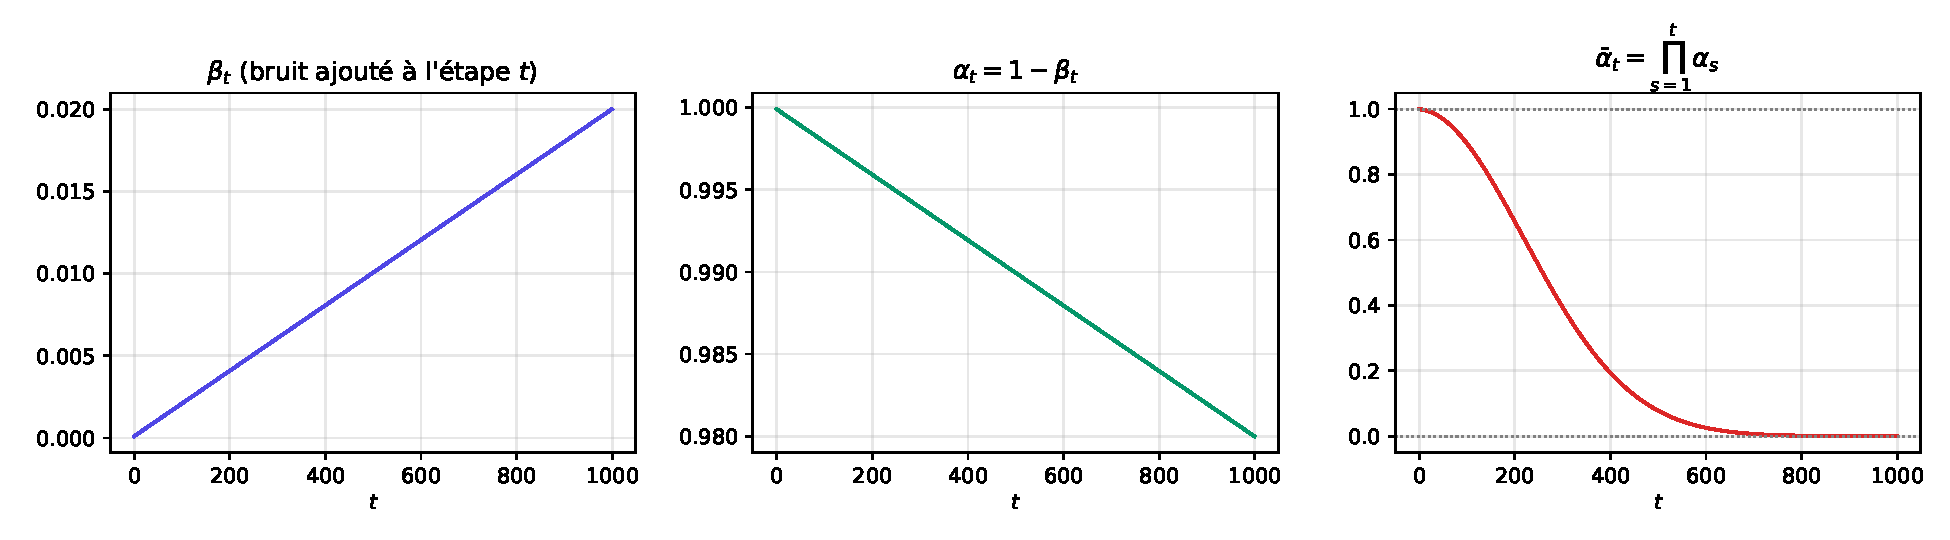
\includegraphics[width=\textwidth]{figures/noise_schedule.pdf}
\caption{Schedule de bruit linéaire ($T=1000$, $\beta_1=10^{-4}$, $\beta_T=2\times10^{-2}$). Notez
comment $\bar\alpha_t$ (produit cumulé) chute rapidement autour de $t \approx 200$–$400$ bien que
$\beta_t$ croisse linéairement : c'est un effet cumulatif, pas une propriété de $\beta_t$ lui-même.}
\label{fig:noise-schedule}
\end{figure}

\begin{figure}[h]
\centering
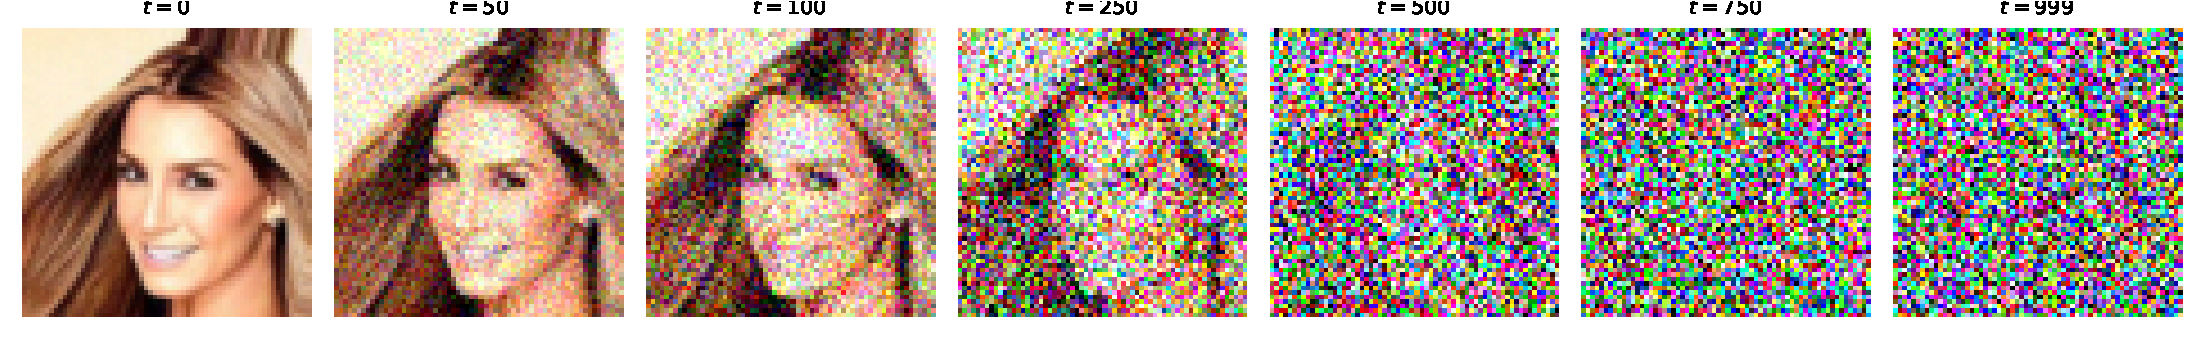
\includegraphics[width=\textwidth]{figures/forward_diffusion.pdf}
\caption{Application de la formule~\eqref{eq:qsample} à une vraie image de visage (CelebA-Dialog), pour
plusieurs valeurs de $t$. L'image reste reconnaissable jusque vers $t\approx 250$, puis se dégrade
rapidement en bruit pur — cohérent avec la chute de $\bar\alpha_t$ observée figure~\ref{fig:noise-schedule}.}
\label{fig:forward-diffusion}
\end{figure}

\section{Le processus inverse}

Défaire le bruitage revient, en théorie, à calculer $q(x_{t-1} \mid x_t)$ — mais cette distribution
dépend de $q(x_{t-1} \mid x_t, x_0)$, donc de $x_0$, que l'on ne connaît justement pas au moment de la
génération (c'est précisément ce qu'on cherche à produire). L'idée du DDPM est d'\textbf{approcher}
cette distribution inconnue par une gaussienne paramétrée :
\begin{equation}
    p_\theta(x_{t-1} \mid x_t) = \mathcal{N}\!\left(x_{t-1};\ \mu_\theta(x_t, t),\ \Sigma_\theta(x_t, t)\right)
\end{equation}
où $\mu_\theta$ est calculée par un réseau de neurones (le U-Net, chapitre~\ref{chap:architecture}), et
où $\Sigma_\theta$ est souvent fixée (non apprise) à $\sigma_t^2 I$ avec $\sigma_t^2 = \beta_t$.

\subsection{Que doit prédire le réseau ?}

Une observation cruciale simplifie tout : on peut montrer (Ho et al., 2020) que la moyenne optimale
$\mu_\theta$ s'exprime naturellement en fonction du \textbf{bruit} $\varepsilon$ qui a été ajouté à
$x_0$ pour produire $x_t$ (équation~\eqref{eq:qsample}) :
\begin{equation}
    \mu_\theta(x_t, t) = \frac{1}{\sqrt{\alpha_t}}\left(x_t - \frac{\beta_t}{\sqrt{1-\bar\alpha_t}}\,\varepsilon_\theta(x_t, t)\right)
\end{equation}
où $\varepsilon_\theta(x_t, t)$ est la sortie du réseau de neurones : \textbf{au lieu de prédire
directement $x_{t-1}$ ou $\mu_\theta$, le réseau apprend à prédire le bruit $\varepsilon$}. C'est un
choix de paramétrisation, pas une nécessité mathématique, mais Ho et al. montrent empiriquement qu'il
conduit à un entraînement bien plus stable et à de meilleurs résultats.

\begin{intuition}
Demander au réseau \og quelle image propre vois-tu dans ce bruit ? \fg\ est une question difficile et
mal posée à haut niveau de bruit (beaucoup d'images propres sont compatibles avec un $x_t$ très
bruité). Demander \og quel bruit a été ajouté ? \fg\ est une question plus simple et mieux posée :
le réseau n'a qu'à reconnaître le \emph{motif de bruit}, une tâche plus locale et plus uniforme sur
toute la plage de $t$.
\end{intuition}

Une fois qu'on a $\mu_\theta$, générer une étape du reverse process consiste à tirer :
\begin{equation}
    \label{eq:psample}
    x_{t-1} = \frac{1}{\sqrt{\alpha_t}}\left(x_t - \frac{\beta_t}{\sqrt{1-\bar\alpha_t}}\,\varepsilon_\theta(x_t, t)\right) + \sigma_t z, \qquad z \sim \mathcal{N}(0, I) \text{ si } t>0 \text{, sinon } z=0
\end{equation}

\section{La fonction de perte}

\subsection{Dérivation (aperçu)}

Comme pour un VAE, on entraîne $p_\theta$ en maximisant une borne inférieure de la log-vraisemblance
(l'ELBO), qui se décompose en une somme de termes de divergence de Kullback-Leibler entre
$q(x_{t-1}\mid x_t, x_0)$ (calculable en forme close) et $p_\theta(x_{t-1}\mid x_t)$, pour chaque $t$.
Chacun de ces termes, une fois la paramétrisation en $\varepsilon_\theta$ substituée, se réduit à une
erreur quadratique pondérée entre le bruit réel et le bruit prédit. La dérivation complète est
disponible dans \cite{ho2020ddpm} ; nous n'en retenons ici que le résultat final.

\subsection{La loss simplifiée}

Ho et al. montrent que retirer les poids issus de la dérivation théorique (c'est-à-dire utiliser une
simple MSE non pondérée) donne, en pratique, de \textbf{meilleurs} résultats visuels :
\begin{equation}
    \boxed{\mathcal{L}_{\text{simple}}(\theta) = \mathbb{E}_{t,\, x_0,\, \varepsilon}\left[\left\lVert \varepsilon - \varepsilon_\theta\!\left(\sqrt{\bar\alpha_t}\,x_0 + \sqrt{1-\bar\alpha_t}\,\varepsilon,\ t\right) \right\rVert^2\right]}
\end{equation}
avec $t \sim \mathcal{U}\{1,\dots,T\}$ et $\varepsilon \sim \mathcal{N}(0,I)$ tirés indépendamment pour
chaque exemple d'entraînement. C'est cette loss, remarquablement simple à implémenter (une MSE entre
deux tenseurs), qui est utilisée dans ce projet.

\section{Algorithmes}

\begin{codebox}[title=Algorithme 1 : Entraînement]
\textbf{répéter jusqu'à convergence :}
\begin{enumerate}[nosep]
    \item tirer $x_0 \sim p_{\text{data}}$ (un batch d'images réelles)
    \item tirer $t \sim \mathcal{U}\{1, \dots, T\}$
    \item tirer $\varepsilon \sim \mathcal{N}(0, I)$
    \item calculer $x_t = \sqrt{\bar\alpha_t}\,x_0 + \sqrt{1-\bar\alpha_t}\,\varepsilon$
    \item calculer la loss $\lVert \varepsilon - \varepsilon_\theta(x_t, t) \rVert^2$ et rétropropager
\end{enumerate}
\end{codebox}

\begin{codebox}[title=Algorithme 2 : Génération (sampling)]
\begin{enumerate}[nosep]
    \item tirer $x_T \sim \mathcal{N}(0, I)$
    \item \textbf{pour} $t = T, T-1, \dots, 1$ \textbf{faire}
    \begin{enumerate}[nosep]
        \item calculer $\varepsilon_\theta(x_t, t)$ avec le réseau entraîné
        \item calculer $x_{t-1}$ via l'équation~\eqref{eq:psample}
    \end{enumerate}
    \item retourner $x_0$
\end{enumerate}
\end{codebox}

\begin{remarque}
Contrairement à l'entraînement (un seul $t$ tiré au hasard par exemple, très rapide), la
\textbf{génération} nécessite $T$ appels séquentiels au réseau — c'est le coût principal des DDPM en
pratique, et la motivation première de méthodes comme le flow matching
(chapitre~\ref{chap:flow}) ou les schémas d'échantillonnage accélérés (DDIM, etc.), qui visent à
réduire ce nombre d'étapes.
\end{remarque}

\section{Conditionnement par texte et classifier-free guidance}
\label{sec:cfg}

Jusqu'ici, $\varepsilon_\theta(x_t, t)$ ne dépend que de l'image bruitée et du temps : le modèle est
\emph{inconditionnel}, il génère \og un visage plausible \fg\ sans contrôle sur son contenu. Pour du
text-to-image, on conditionne le réseau sur une représentation du texte $c$ (obtenue par un encodeur de
texte, voir section~\ref{sec:clip}) :
\begin{equation}
    \varepsilon_\theta(x_t, t, c)
\end{equation}
Le mécanisme précis d'injection de $c$ dans le réseau (cross-attention) est détaillé au
chapitre~\ref{chap:architecture}.

\subsection{Classifier-free guidance}

Conditionner naïvement ne garantit pas que le modèle \emph{suive fortement} le texte : rien n'empêche
le réseau d'apprendre à ignorer partiellement $c$ si les images d'entraînement sont déjà assez
prévisibles sans lui. Le \emph{classifier-free guidance} (Ho \& Salimans, 2022) \cite{ho2022cfg} est une
technique simple et efficace pour renforcer cette influence.

\textbf{À l'entraînement}, on remplace aléatoirement le conditionnement $c$ par un token vide
$\varnothing$ avec une probabilité $p_{\text{uncond}}$ (typiquement $10\,\%$), de sorte que le même
réseau apprenne \textbf{à la fois} $\varepsilon_\theta(x_t, t, c)$ (conditionnel) \textbf{et}
$\varepsilon_\theta(x_t, t, \varnothing)$ (inconditionnel).

\textbf{À la génération}, on combine les deux prédictions avec un facteur d'amplification
$w \geq 1$ (le \emph{guidance scale}) :
\begin{equation}
    \tilde\varepsilon_\theta(x_t, t, c) = \varepsilon_\theta(x_t, t, \varnothing) + w \cdot \big(\varepsilon_\theta(x_t, t, c) - \varepsilon_\theta(x_t, t, \varnothing)\big)
\end{equation}

\begin{intuition}
Le terme $\varepsilon_\theta(x_t,t,c) - \varepsilon_\theta(x_t,t,\varnothing)$ est la direction
\og apportée par le texte \fg\ : la différence entre ce que le modèle ferait avec et sans
conditionnement. L'amplifier par $w > 1$ exagère cette direction, produisant des images qui suivent le
prompt plus fidèlement — au prix, si $w$ est trop grand, d'une perte de diversité et d'artefacts
visuels (le modèle \og sur-corrige \fg).
\end{intuition}

Ce mécanisme de dropout du conditionnement à l'entraînement est implémenté dans ce projet (voir
chapitre~\ref{chap:project}) ; l'application du facteur $w$ au moment du sampling est un point
d'extension naturel du code fourni.

\chapter{Flow Matching}
\label{chap:flow}

Le \emph{Conditional Flow Matching} (Lipman et al., 2023) \cite{lipman2023flow} propose une
reformulation du même principe que la diffusion — transformer progressivement du bruit en donnée — mais
en des termes plus directs, empruntés à la théorie des équations différentielles ordinaires (ODE)
plutôt qu'aux chaînes de Markov gaussiennes.

\section{Des chemins discrets aux chemins continus}

Le DDPM construit implicitement un chemin \emph{stochastique} entre $x_0$ (donnée) et $x_T$ (bruit),
en $T$ pas discrets, chacun ajoutant un peu de bruit aléatoire. Le flow matching part d'une idée plus
simple : et si on définissait directement un chemin \textbf{déterministe et continu} entre les deux ?

\begin{definition}[Chemin d'interpolation linéaire]
Pour $t \in [0, 1]$ continu (notez le changement de convention par rapport au DDPM : ici $t=0$ est la
donnée et $t=1$ est le bruit), on définit :
\begin{equation}
    \label{eq:flow-interp}
    x_t = (1-t)\, x_0 + t\, x_1, \qquad x_0 \sim p_{\text{data}}, \quad x_1 \sim \mathcal{N}(0, I)
\end{equation}
\end{definition}

C'est un simple segment de droite dans l'espace des images : à $t=0$ on est exactement sur la donnée,
à $t=1$ exactement sur le bruit, et entre les deux, un mélange linéaire.

\begin{figure}[h]
\centering
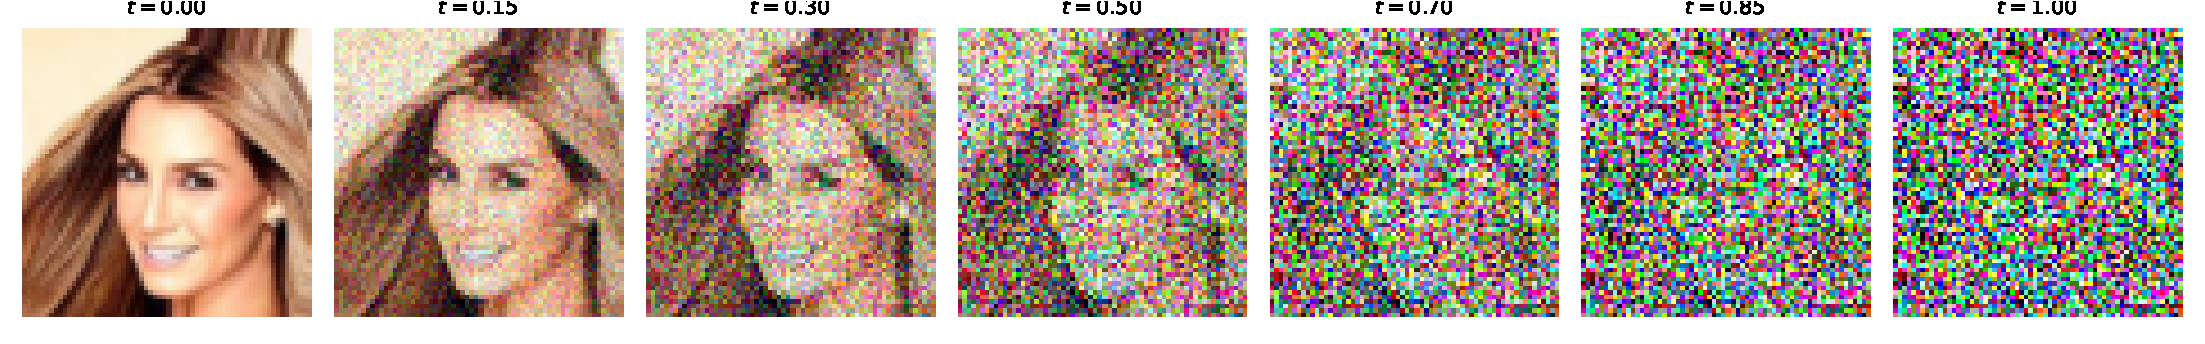
\includegraphics[width=\textwidth]{figures/flow_interpolation.pdf}
\caption{Interpolation linéaire~\eqref{eq:flow-interp} entre une image réelle et un bruit fixé, pour
plusieurs valeurs de $t$. À comparer avec la figure~\ref{fig:forward-diffusion} (bruitage DDPM) : la
dégradation est ici parfaitement régulière et prévisible, puisque déterministe.}
\label{fig:flow-interp}
\end{figure}

\begin{figure}[h]
\centering
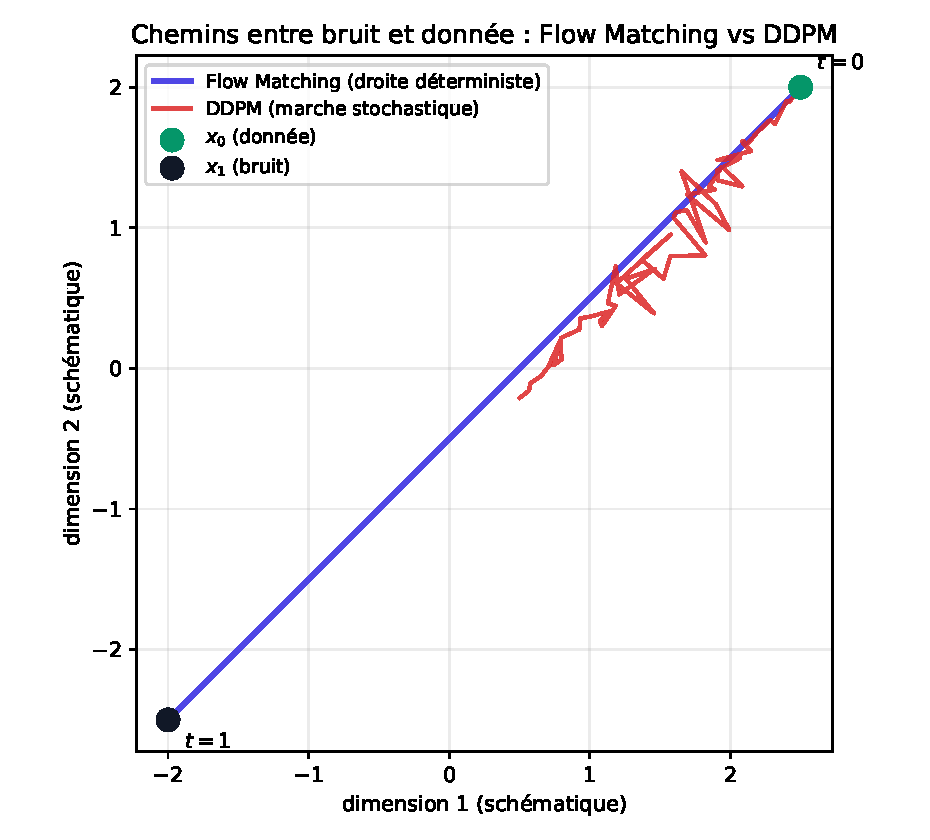
\includegraphics[width=0.72\textwidth]{figures/ddpm_vs_flow_paths.pdf}
\caption{Illustration schématique (exemple jouet en 2D, sans rapport avec le vrai espace des images)
de la différence entre les deux processus : le flow matching suit une trajectoire rectiligne et
déterministe, le DDPM une marche bruitée qui suit le même schedule cumulatif $\bar\alpha_t$ mais avec
des écarts aléatoires à chaque pas.}
\label{fig:paths-comparison}
\end{figure}

\section{Le champ de vitesse}

Dériver l'équation~\eqref{eq:flow-interp} par rapport à $t$ donne la \textbf{vélocité} du point le long
du chemin :
\begin{equation}
    \frac{dx_t}{dt} = x_1 - x_0
\end{equation}
Remarquez que cette quantité ne dépend pas de $t$ : elle est \textbf{constante le long de tout le
segment} — c'est la vitesse d'un mouvement rectiligne uniforme entre $x_0$ et $x_1$.

\begin{definition}[Objectif du flow matching]
On entraîne un réseau $v_\theta(x, t)$ à prédire cette vélocité, pour n'importe quel point $x$ sur
n'importe quel chemin, à n'importe quel instant $t$ :
\begin{equation}
    \boxed{\mathcal{L}_{\text{FM}}(\theta) = \mathbb{E}_{t \sim \mathcal{U}[0,1],\ x_0 \sim p_{\text{data}},\ x_1 \sim \mathcal{N}(0,I)}\left[\left\lVert v_\theta\big((1-t)x_0 + t x_1,\ t\big) - (x_1 - x_0) \right\rVert^2\right]}
\end{equation}
\end{definition}

\begin{intuition}
Chaque paire $(x_0, x_1)$ tirée pendant l'entraînement définit \emph{son propre} segment de droite, de
sa propre vélocité constante $x_1 - x_0$. Le réseau ne voit jamais un segment entier : à chaque exemple
d'entraînement, il ne voit qu'un point $x_t$ tiré sur \emph{un} segment, avec la consigne \og la
vélocité ici doit valoir $x_1 - x_0$ \fg. En moyennant sur des millions de tels segments, le réseau
apprend, pour toute région de l'espace, une vélocité \emph{moyenne} qui tient compte de tous les
segments qui passent à proximité — c'est ce qui permet, à la génération, de suivre un chemin cohérent
même en partant d'un point de bruit qui n'a jamais été vu exactement pendant l'entraînement (voir la
figure~\ref{fig:vector-field}).
\end{intuition}

\begin{figure}[h]
\centering
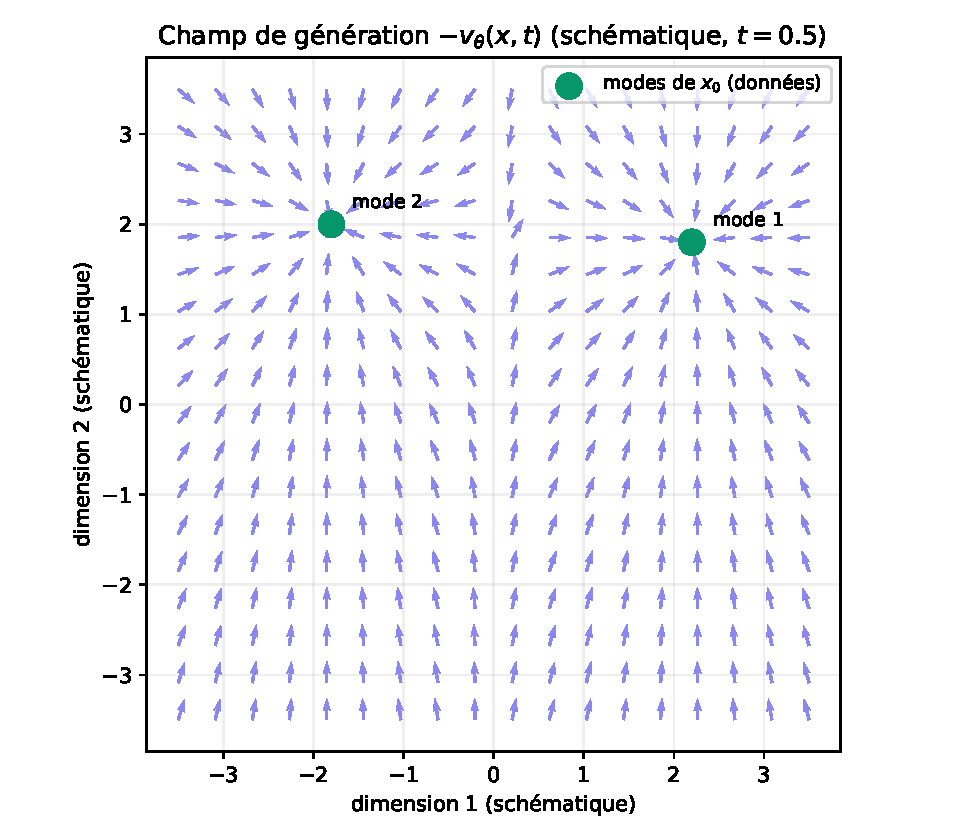
\includegraphics[width=0.7\textwidth]{figures/vector_field.pdf}
\caption{Champ de vitesse appris (schématique, exemple 2D jouet à deux modes de données) : à chaque
point de l'espace, le réseau prédit une direction. Ici on affiche $-v_\theta$, le sens réellement suivi
pendant la génération, qui converge naturellement vers les modes de la distribution de données.}
\label{fig:vector-field}
\end{figure}

\section{Génération : résoudre une équation différentielle}

Une fois $v_\theta$ entraîné, générer une image consiste à résoudre l'équation différentielle ordinaire
\begin{equation}
    \frac{dx_t}{dt} = v_\theta(x_t, t)
\end{equation}
en partant de $x_1 \sim \mathcal{N}(0, I)$ (bruit pur, $t=1$) et en intégrant \textbf{à rebours}
jusqu'à $t=0$. Le schéma numérique le plus simple, l'\textbf{Euler explicite}, discrétise cette
intégration en $N$ pas de taille $dt = 1/N$ :
\begin{equation}
    x_{t - dt} = x_t - dt \cdot v_\theta(x_t, t)
\end{equation}

\begin{codebox}[title=Algorithme : Génération par Flow Matching (Euler explicite)]
\begin{enumerate}[nosep]
    \item tirer $x_1 \sim \mathcal{N}(0, I)$ ; poser $t \leftarrow 1$, $dt \leftarrow 1/N$
    \item \textbf{répéter $N$ fois :}
    \begin{enumerate}[nosep]
        \item calculer $v_\theta(x_t, t)$ avec le réseau entraîné
        \item $x_{t-dt} \leftarrow x_t - dt \cdot v_\theta(x_t, t)$ ; $t \leftarrow t - dt$
    \end{enumerate}
    \item retourner $x_0$
\end{enumerate}
\end{codebox}

\begin{remarque}
Contrairement au reverse process du DDPM (équation~\eqref{eq:psample}), \textbf{aucun bruit aléatoire
n'est réinjecté} à chaque étape : la trajectoire complète est entièrement déterminée par le point de
départ $x_1$ et le réseau $v_\theta$. Deux générations avec le même $x_1$ produisent exactement la
même image. C'est une différence qualitative importante avec le DDPM, dont chaque étape du reverse
process est stochastique.
\end{remarque}

\section{Pourquoi (souvent) moins d'étapes suffisent}

Le chemin appris par le flow matching est, par construction, rectiligne au niveau de chaque exemple
d'entraînement individuel, et le champ moyen résultant tend à rester relativement \og droit \fg. Un
solveur ODE comme Euler explicite approxime d'autant mieux une trajectoire qu'elle est proche d'une
droite : l'erreur de discrétisation d'Euler est en $O(dt)$ par pas, et une trajectoire rectiligne ne
requiert presque aucune correction de direction entre deux pas consécutifs. C'est ce qui explique
pourquoi, en pratique, le flow matching atteint souvent une qualité comparable avec beaucoup moins de
pas de génération ($N \approx 20$–$50$) qu'un DDPM classique ($T \approx 250$–$1000$), bien que ce ne
soit pas une garantie absolue et que cela dépende de la complexité de la distribution de données.

\section{Diffusion et flow matching : une même famille}

Il est utile de noter que DDPM et flow matching, malgré des présentations mathématiques différentes
(chaînes de Markov gaussiennes contre ODE continues), appartiennent tous deux à la famille plus large
des \emph{modèles à transport continu de distribution}, et peuvent même être reliés formellement (le
flow matching avec un chemin gaussien bien choisi retrouve une formulation proche du DDPM en temps
continu). Le tableau~\ref{tab:comparison} résume les différences pratiques entre les deux
implémentations telles qu'utilisées dans ce projet.

\begin{table}[h]
\centering
\begin{tabular}{@{}lll@{}}
\toprule
& \textbf{DDPM} & \textbf{Flow Matching} \\
\midrule
Variable temporelle & $t \in \{0, \dots, T-1\}$ discret & $t \in [0,1]$ continu \\
Construction de $x_t$ & schedule $\bar\alpha_t$ (non-linéaire) & interpolation linéaire \\
Sortie du réseau & bruit $\varepsilon_\theta$ & vélocité $v_\theta$ \\
Cible de la loss & $\varepsilon$ (bruit ajouté) & $x_1 - x_0$ (constant sur le chemin) \\
Génération & stochastique (bruit à chaque pas) & déterministe (ODE) \\
Nb. d'étapes typique & 250 -- 1000 & 20 -- 50 \\
\bottomrule
\end{tabular}
\caption{Comparaison pratique des deux approches implémentées dans ce projet.}
\label{tab:comparison}
\end{table}

\chapter{Architecture : le réseau qui apprend à débruiter}
\label{chap:architecture}

Les deux chapitres précédents ont défini \emph{ce que} le réseau doit apprendre à prédire
($\varepsilon_\theta$ pour le DDPM, $v_\theta$ pour le flow matching). Ce chapitre décrit \emph{quel}
réseau remplit ce rôle. Un point essentiel structure tout ce chapitre :

\begin{intuition}
Le réseau ignore totalement s'il fait de la diffusion ou du flow matching. Il résout un seul et même
problème de régression : \og étant donné une image $x_t$ dégradée, un temps $t$, et éventuellement un
texte, produis un tenseur de même forme que $x_t$ \fg. Seule l'interprétation de cette sortie (un
bruit ou une vélocité) et la façon dont $x_t$ a été construit diffèrent entre les deux approches. C'est
pourquoi une \textbf{seule et même architecture} — le U-Net décrit ici — est réutilisée sans aucune
modification pour les deux méthodes dans ce projet.
\end{intuition}

\section{Le choix de l'architecture U-Net}

Le réseau doit accomplir une tâche de \emph{traduction image-à-image} : recevoir une image bruitée et
produire une sortie de même résolution spatiale. L'architecture U-Net (Ronneberger et al., 2015,
initialement conçue pour la segmentation d'images médicales) est bien adaptée à ce type de tâche :

\begin{itemize}
    \item une branche \textbf{descendante} (\emph{encoder}) réduit progressivement la résolution
    spatiale tout en augmentant le nombre de canaux, extrayant des caractéristiques de plus en plus
    abstraites ;
    \item une branche \textbf{montante} (\emph{decoder}), symétrique, restaure progressivement la
    résolution d'origine ;
    \item des \textbf{connexions résiduelles} (\emph{skip connections}) relient chaque étage de la
    descente à l'étage de la montée de même résolution, permettant de préserver les détails fins qui
    seraient sinon perdus dans le goulot d'étranglement central.
\end{itemize}

\section{Vue d'ensemble du réseau}

La figure~\ref{fig:unet-architecture} présente l'architecture complète telle qu'implémentée dans ce
projet (configuration par défaut : canaux $[64, 128, 256, 256]$, résolutions $64 \to 32 \to 16 \to 8$).

\begin{figure}[p]
\centering
\resizebox{\textwidth}{!}{% Schéma d'architecture du U-Net partagé (src/backend/shared/unet.py).
% Fidèle à la configuration par défaut : base_channels=64,
% channel_multipliers=(1,2,4,4) -> canaux [64,128,256,256],
% résolutions 64->32->16->8, cross-attention aux étages 32/16/8.
\begin{tikzpicture}[
    font=\small,
    block/.style={draw, rounded corners, minimum width=2.6cm, minimum height=0.85cm, align=center, fill=blue!6},
    attn/.style={draw, rounded corners, minimum width=2.6cm, minimum height=0.65cm, align=center, fill=orange!12},
    io/.style={draw, rounded corners, minimum width=2.6cm, minimum height=0.7cm, align=center, fill=green!8},
    arr/.style={-Stealth, thick},
    skiparr/.style={-Stealth, thick, dashed, gray},
    timearr/.style={-Stealth, thick, purple},
    textarr/.style={-Stealth, thick, orange!80!black},
]

% --- Colonne d'entrée / sortie (gauche) ---
\node[io] (xin) at (0, 0) {$x_t$ \\ $(3,64,64)$};
\node[block] (convin) at (0, -1.4) {Conv$_{3\times3}$ in};

% --- Down path (espacement horizontal augmenté pour laisser respirer les
%     labels downsample/upsample et les flèches d'injection du temps) ---
\node[block] (d0) at (0, -3.0) {ResBlock $\times2$ \\ 64ch, 64$\times$64};
\node[block] (d1) at (3.6, -4.8) {ResBlock $\times2$ \\ 128ch, 32$\times$32};
\node[attn]  (a1) at (3.6, -5.75) {CrossAttn};
\node[block] (d2) at (7.2, -7.2) {ResBlock $\times2$ \\ 256ch, 16$\times$16};
\node[attn]  (a2) at (7.2, -8.15) {CrossAttn};

% --- Bottleneck ---
\node[block] (bn) at (10.8, -9.6) {ResBlock \\ 256ch, 8$\times$8};
\node[attn]  (abn) at (10.8, -10.55) {CrossAttn};
\node[block] (bn2) at (10.8, -11.4) {ResBlock};

% --- Up path (symétrique) ---
\node[block] (u2) at (14.4, -7.2) {ResBlock $\times2$ \\ 256ch, 16$\times$16};
\node[attn]  (au2) at (14.4, -8.15) {CrossAttn};
\node[block] (u1) at (18.0, -4.8) {ResBlock $\times2$ \\ 128ch, 32$\times$32};
\node[attn]  (au1) at (18.0, -5.75) {CrossAttn};
\node[block] (u0) at (21.6, -3.0) {ResBlock $\times2$ \\ 64ch, 64$\times$64};

\node[block] (convout) at (21.6, -1.4) {Conv$_{3\times3}$ out};
\node[io] (xout) at (21.6, 0) {$\varepsilon_\theta$ ou $v_\theta$ \\ $(3,64,64)$};

% --- Flux principal ---
\draw[arr] (xin) -- (convin);
\draw[arr] (convin) -- (d0);
\draw[arr] (d0) -- node[above,sloped,font=\tiny]{downsample} (d1);
\draw[arr] (d1) -- (a1);
\draw[arr] (a1) -- node[above,sloped,font=\tiny]{downsample} (d2);
\draw[arr] (d2) -- (a2);
\draw[arr] (a2) -- node[above,sloped,font=\tiny]{downsample} (bn);
\draw[arr] (bn) -- (abn);
\draw[arr] (abn) -- (bn2);
\draw[arr] (bn2) -- node[above,sloped,font=\tiny]{upsample} (u2);
\draw[arr] (u2) -- (au2);
\draw[arr] (au2) -- node[above,sloped,font=\tiny]{upsample} (u1);
\draw[arr] (u1) -- (au1);
\draw[arr] (au1) -- node[above,sloped,font=\tiny]{upsample} (u0);
\draw[arr] (u0) -- (convout);
\draw[arr] (convout) -- (xout);

% --- Skip connections (concaténation down -> up, même résolution) ---
\draw[skiparr] (d0.east) to[bend left=15] node[above,font=\tiny]{skip} (u0.west);
\draw[skiparr] (a1.east) to[bend left=15] node[above,font=\tiny]{skip} (au1.west);
\draw[skiparr] (a2.east) to[bend left=15] node[above,font=\tiny]{skip} (au2.west);

% --- Injection du temps t : dans CHAQUE ResBlock ---
\node[draw, rounded corners, fill=purple!10, minimum width=2.6cm, minimum height=0.7cm, align=center] (temb) at (10.8, -1.4) {$t \to$ sinusoidal \\ $+$ MLP $\to \vec{t}$};
\foreach \blk in {d0, d1, d2, bn, bn2, u2, u1, u0} {
  \draw[timearr] (temb) -- (\blk);
}

% --- Injection du texte : cross-attention sur chaque bloc d'attention ---
\node[draw, rounded corners, fill=orange!10, minimum width=2.8cm, minimum height=0.7cm, align=center] (text) at (10.8, -13.0) {CLIP texte (gelé) \\ $(77, 512)$};
\foreach \blk in {a1, a2, abn, au2, au1} {
  \draw[textarr] (text) -- (\blk);
}

\end{tikzpicture}
}
\caption{Architecture complète du U-Net partagé. Le flux principal (image) traverse le réseau en
forme de U (traits noirs pleins). Le temps $t$ (violet) est injecté dans \emph{chaque} bloc résiduel,
à toutes les résolutions. Le texte (orange), encodé par CLIP gelé, est injecté par cross-attention aux
résolutions $32\times32$, $16\times16$ et au goulot d'étranglement $8\times8$ — pas à la résolution la
plus fine $64\times64$, où le coût quadratique de l'attention serait trop élevé pour le bénéfice
apporté. Les connexions en pointillés gris sont les skip connections entre étages de même résolution.}
\label{fig:unet-architecture}
\end{figure}

Trois mécanismes assemblent ce réseau ; nous les détaillons dans le reste du chapitre :
\begin{enumerate}
    \item l'\textbf{injection du temps} $t$ (section~\ref{sec:time-embed}), qui indique au réseau à
    quel niveau de dégradation il travaille, à chaque étage ;
    \item le \textbf{bloc résiduel} (\emph{ResBlock}, section~\ref{sec:resblock}), l'unité de base
    répétée à chaque étage ;
    \item l'\textbf{injection du texte} par cross-attention (section~\ref{sec:cross-attn}), qui permet
    au réseau de conditionner sa prédiction sur une description en langage naturel.
\end{enumerate}

\section{Encoder le temps : l'embedding sinusoïdal}
\label{sec:time-embed}

Le réseau reçoit $t$ (un simple entier, ou un flottant continu pour le flow matching) : un scalaire
brut est un signal pauvre et mal exploitable par des couches de convolution. On le transforme d'abord
en un vecteur riche, via un \emph{encodage sinusoïdal} — le même principe que le positional encoding
des Transformers (Vaswani et al., 2017) :
\begin{equation}
    \text{PE}(t, 2i) = \sin\!\left(\frac{t}{10000^{2i/d}}\right), \qquad
    \text{PE}(t, 2i+1) = \cos\!\left(\frac{t}{10000^{2i/d}}\right)
\end{equation}
où $d$ est la dimension de l'encodage et $i \in \{0, \dots, d/2-1\}$ indexe des fréquences
décroissantes. Ce vecteur est ensuite passé dans un petit MLP (\texttt{Linear} $\to$ SiLU $\to$
\texttt{Linear}) pour donner au réseau la capacité d'en tirer une représentation utile à ses propres
besoins internes.

\begin{figure}[h]
\centering
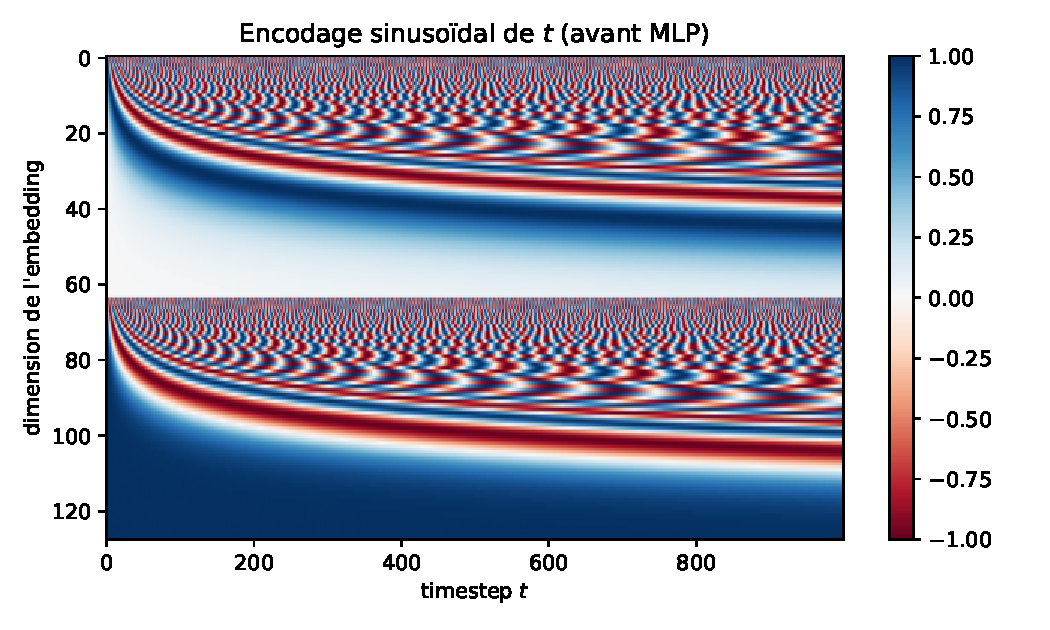
\includegraphics[width=0.75\textwidth]{figures/time_embedding.pdf}
\caption{Visualisation de l'encodage sinusoïdal brut (avant le MLP) pour $d=128$ et $t \in [0, 1000)$.
Chaque ligne horizontale oscille à sa propre fréquence : les dimensions du haut de chaque moitié
(sinus/cosinus) oscillent rapidement (hautes fréquences), celles du bas lentement (basses fréquences).
La combinaison de toutes ces fréquences donne, pour chaque valeur de $t$, une \og signature \fg\ unique
et continue (deux $t$ proches ont des colonnes visuellement proches dans cette figure).}
\label{fig:time-embedding}
\end{figure}

\begin{intuition}
C'est l'analogue d'une horloge à plusieurs aiguilles tournant à des vitesses différentes (secondes,
minutes, heures) : en lisant la position de toutes les aiguilles simultanément, on identifie un instant
précis. Ici, chaque dimension de l'embedding est une \og aiguille \fg\ tournant à sa fréquence propre en
fonction de $t$.
\end{intuition}

Le vecteur final, noté $\vec t \in \mathbb{R}^{d_{\text{temps}}}$ (dimension $512$ dans ce projet),
n'est \textbf{pas} donné une seule fois en entrée du réseau : il est ré-injecté dans \emph{chaque}
ResBlock, à \emph{chaque} étage de résolution (flèches violettes de la figure~\ref{fig:unet-architecture}).

\section{Le bloc résiduel (ResBlock)}
\label{sec:resblock}

C'est l'unité de calcul de base, répétée à chaque étage du U-Net. Son rôle est double : extraire des
caractéristiques locales de l'image par convolution, et moduler ce calcul en fonction du temps $\vec t$.

\begin{equation}
\begin{aligned}
    h &= \text{Conv}_{3\times3}\big(\text{SiLU}(\text{GroupNorm}(x))\big) \\
    h &= h + \text{Linear}(\vec t)_{\ \text{broadcast sur } H,W} \\
    h &= \text{Conv}_{3\times3}\big(\text{SiLU}(\text{GroupNorm}(h))\big) \\
    \text{sortie} &= h + \text{skip}(x)
\end{aligned}
\end{equation}

où $\text{skip}(x) = x$ si le nombre de canaux ne change pas, et $\text{skip}(x) = \text{Conv}_{1\times1}(x)$
sinon (pour ajuster la dimension avant l'addition résiduelle).

\begin{intuition}
La projection linéaire de $\vec t$, additionnée aux feature maps après la première convolution, agit
comme un \og biais dépendant du contexte \fg : elle décale toutes les activations d'une quantité qui
dépend du niveau de bruit courant, permettant au même jeu de poids de convolution de se comporter
différemment selon que l'on débruite une image très bruitée ($t$ grand) ou presque propre ($t$ petit).
\end{intuition}

La connexion résiduelle ($h + \text{skip}(x)$) suit le principe des ResNets (He et al., 2015) : elle
facilite la propagation du gradient à travers un réseau profond (rappelons que le U-Net complet
comporte des dizaines de ces blocs empilés), en donnant au réseau la possibilité d'apprendre une
simple perturbation de l'entrée plutôt qu'une transformation complète.

\section{Conditionner sur le texte : la cross-attention}
\label{sec:cross-attn}

\subsection{Représenter le texte : CLIP}
\label{sec:clip}

Comprendre du texte libre (grammaire, synonymes, combinaisons d'attributs) demande d'avoir vu une
quantité de langage bien supérieure à ce qu'un jeu de données de quelques centaines de milliers de
légendes peut fournir à un encodeur entraîné \emph{from scratch}. Ce projet réutilise donc un encodeur
de texte \textbf{pré-entraîné et gelé} : le \emph{text encoder} de CLIP (Radford et al., 2021)
\cite{radford2021clip}, dont les poids ne sont \textbf{jamais mis à jour} pendant l'entraînement —
seul le U-Net apprend.

CLIP a été entraîné à aligner des représentations de texte et d'image sur des centaines de millions de
paires (image, légende) : ses embeddings capturent donc déjà des notions visuelles pertinentes
(\og souriant \fg, \og lunettes \fg\ sont représentés de façon cohérente avec leur contenu visuel),
même si CLIP lui-même n'a jamais vu le jeu de données CelebA-Dialog. Une phrase en entrée produit une
séquence d'embeddings, un par token :
\begin{equation}
    \text{texte} \xrightarrow{\ \text{CLIP (gelé)}\ } \text{embed} \in \mathbb{R}^{77 \times 512}
\end{equation}
(77 étant la longueur de séquence maximale standard de CLIP, avec padding pour les phrases plus courtes).

\subsection{Le mécanisme de cross-attention}

Une fois le texte encodé, comment le U-Net l'utilise-t-il ? La réponse est l'\textbf{attention croisée}
(\emph{cross-attention}), le même mécanisme central des Transformers (Vaswani et al., 2017), mais
appliqué entre deux modalités différentes (image et texte) plutôt qu'au sein d'une seule séquence.

\begin{figure}[h]
\centering
\resizebox{0.85\textwidth}{!}{% Schéma du mécanisme de cross-attention texte -> image (src/backend/shared/unet_blocks.py, CrossAttentionBlock).
\begin{tikzpicture}[
    font=\small,
    block/.style={draw, rounded corners, minimum width=2.4cm, minimum height=0.8cm, align=center},
    arr/.style={-Stealth, thick},
]

\node[block, fill=blue!8] (img) at (0, 3) {feature map image \\ $(B, C, H, W)$};
\node[block, fill=blue!8] (flat) at (0, 1.6) {aplatie en séquence \\ $(B, HW, C)$};
\node[block, fill=blue!15] (q) at (0, 0.2) {$Q = W_Q \cdot h$ \\ $(B, HW, C)$};

\node[block, fill=orange!8] (txt) at (7, 3) {embeddings CLIP \\ $(B, 77, 512)$};
\node[block, fill=orange!15] (k) at (5.5, 1.6) {$K = W_K \cdot \text{texte}$};
\node[block, fill=orange!15] (v) at (8.5, 1.6) {$V = W_V \cdot \text{texte}$};

\node[block, fill=green!12, minimum width=5cm] (attn) at (3.5, -1.4) {$\text{Attention}(Q,K,V) = \text{softmax}\!\left(\dfrac{QK^\top}{\sqrt{d}}\right) V$};

\node[block, fill=blue!8] (out) at (3.5, -3) {$+$ résiduel, reshape \\ $(B, C, H, W)$};

\draw[arr] (img) -- (flat);
\draw[arr] (flat) -- (q);
\draw[arr] (txt) -- (k);
\draw[arr] (txt) -- (v);
\draw[arr] (q) -- (attn);
\draw[arr] (k) -- (attn);
\draw[arr] (v) -- (attn);
\draw[arr] (attn) -- (out);
\draw[arr, dashed, gray] (img.south) to[bend right=35] node[left, font=\tiny]{skip} (out.west);

\end{tikzpicture}
}
\caption{Mécanisme de cross-attention texte $\to$ image utilisé dans chaque bloc \texttt{CrossAttentionBlock}
du U-Net. Les positions spatiales de la feature map image forment les requêtes (\emph{queries}) ; les
tokens du texte fournissent les clés (\emph{keys}) et valeurs (\emph{values}).}
\label{fig:cross-attention}
\end{figure}

Concrètement, à une résolution donnée, la feature map image de forme $(B, C, H, W)$ est aplatie en une
séquence de $H \times W$ \og pixels \fg, chacun projeté en une requête $Q$. Le texte fournit les clés
$K$ et valeurs $V$. L'attention standard est alors calculée :
\begin{equation}
    \text{Attention}(Q, K, V) = \text{softmax}\!\left(\frac{QK^\top}{\sqrt{d}}\right) V
\end{equation}

\begin{intuition}
Chaque position spatiale de l'image \og interroge \fg\ tous les mots de la phrase et récupère une
combinaison pondérée de l'information qu'ils encodent, pondérée par leur pertinence pour cette
position précise. Par exemple, les positions spatiales correspondant à la zone de la bouche
apprendront, au fil de l'entraînement, à accorder plus de poids aux tokens liés au sourire si la
légende en mentionne un.
\end{intuition}

Comme pour le ResBlock, une connexion résiduelle est appliquée : la sortie de l'attention est
\textbf{ajoutée} à la feature map d'entrée plutôt que de la remplacer, ce qui permet au réseau
d'apprendre progressivement à quel point utiliser l'information textuelle à cet endroit précis du
réseau.

\subsection{Où placer les blocs de cross-attention ?}

Le coût de calcul de l'attention standard est quadratique en le nombre de positions
($O((HW)^2)$) : l'appliquer à la résolution la plus fine ($64\times64 = 4096$ positions) serait
prohibitif. Ce projet suit le choix standard (repris de Stable Diffusion) d'activer la cross-attention
uniquement aux résolutions intermédiaires et basses ($32\times32$, $16\times16$, et le goulot
d'étranglement $8\times8$), où le nombre de positions reste raisonnable tout en donnant au réseau
suffisamment d'occasions d'intégrer l'information textuelle à différentes échelles de représentation.

\chapter{Application : implémentation du projet}
\label{chap:project}

Ce chapitre relie chaque élément théorique des chapitres précédents au code du dépôt
(\texttt{text-\linebreak[1]to-\linebreak[1]image-\linebreak[1]generative-\linebreak[1]models}), une
implémentation \emph{from scratch} en PyTorch, conçue pour tourner entièrement en local sur un Mac
Apple Silicon (accélération MPS).

\section{Choix de conception}

\begin{itemize}
    \item \textbf{Diffusion pixel-space, pas latent-space.} Contrairement à Stable Diffusion, qui
    diffuse dans l'espace latent compressé d'un VAE, ce projet diffuse directement dans l'espace des
    pixels. Ce choix simplifie considérablement l'implémentation (pas de VAE à entraîner ou à
    intégrer) au prix d'une résolution de travail plus faible ($64\times64$), un compromis raisonnable
    pour un objectif pédagogique réalisable en local.
    \item \textbf{Un seul U-Net, deux approches.} Comme expliqué au chapitre~\ref{chap:architecture},
    l'architecture U-Net (\texttt{src/backend/shared/unet.py}) est strictement identique pour le DDPM
    et le flow matching : seule la construction de $x_t$ et l'interprétation de la sortie du réseau
    diffèrent.
    \item \textbf{CLIP gelé.} Le texte est encodé par \texttt{openai/clip-vit-base-patch32}
    (\texttt{transformers}), jamais réentraîné.
\end{itemize}

\section{Le jeu de données : CelebA-Dialog}

Le projet utilise CelebA-Dialog (Jiang et al., 2021) \cite{jiang2021celebadialog}, une extension de
CelebA qui associe à chacune des $202\,599$ images de visages une légende en langage naturel générée à
partir de cinq attributs à échelle graduée (\texttt{Bangs}, \texttt{Eyeglasses}, \texttt{No\_Beard},
\texttt{Smiling}, \texttt{Young}) : par exemple \og \emph{This person is a young smiling woman with
long bangs and no eyeglasses.} \fg\ Ce jeu de données permet un conditionnement textuel plus riche que
de simples labels de classe, sans nécessiter la collecte de vraies légendes humaines pour chaque
image, comme le ferait par exemple COCO Captions.

Le module \texttt{src/backend/shared/dataset.py} (classe \texttt{CelebACaptionDataset}) charge une
paire (image, légende), applique le split officiel train/val/test, et exclut automatiquement les
quelques images sans annotation disponible.

\section{Correspondance théorie $\leftrightarrow$ code}

\begin{table}[h]
\centering
\small
\begin{tabular}{@{}p{5.4cm}p{9.2cm}@{}}
\toprule
\textbf{Concept théorique} & \textbf{Fichier} \\
\midrule
Bruitage forward $q(x_t\mid x_0)$, éq.~\eqref{eq:qsample} & \texttt{src/backend/diffusion/gaussian\_diffusion.py} \newline (\texttt{GaussianDiffusion.q\_sample}) \\
Reverse process, éq.~\eqref{eq:psample} & \texttt{GaussianDiffusion.p\_sample} \\
Interpolation Flow Matching, éq.~\eqref{eq:flow-interp} & \texttt{src/backend/flow\_matching/flow\_matching.py} \newline (\texttt{ConditionalFlowMatching.sample\_xt}) \\
Encodage sinusoïdal du temps & \texttt{src/backend/shared/time\_embedding.py} \\
ResBlock, CrossAttentionBlock & \texttt{src/backend/shared/unet\_blocks.py} \\
U-Net complet & \texttt{src/backend/shared/unet.py} \\
Encodeur texte CLIP gelé & \texttt{src/backend/shared/text\_encoder.py} \\
Loss DDPM (MSE sur le bruit) et training loop & \texttt{src/backend/diffusion/train.py} \\
Loss Flow Matching (MSE sur la vélocité) et training loop & \texttt{src/backend/flow\_matching/train.py} \\
Génération par débruitage itératif (Algo. 2, chap.~\ref{chap:ddpm}) & \texttt{src/backend/diffusion/sample.py} \\
Génération par résolution ODE (Euler explicite) & \texttt{src/backend/flow\_matching/sample.py} \\
Classifier-free guidance (dropout à l'entraînement) & argument \texttt{cfg\_dropout\_prob} des deux \texttt{train.py} \\
\bottomrule
\end{tabular}
\caption{Correspondance entre les notions théoriques du cours et leur implémentation.}
\end{table}

\section{Un exemple de code : la formule fermée du bruitage}

L'équation~\eqref{eq:qsample} se traduit directement en quelques lignes de PyTorch :

\begin{lstlisting}[language=Python]
def q_sample(self, x_0, t, noise=None):
    if noise is None:
        noise = torch.randn_like(x_0)
    sqrt_alphas_cumprod_t = self._extract(self.sqrt_alphas_cumprod, t, x_0.shape)
    sqrt_one_minus_alphas_cumprod_t = self._extract(
        self.sqrt_one_minus_alphas_cumprod, t, x_0.shape
    )
    x_t = sqrt_alphas_cumprod_t * x_0 + sqrt_one_minus_alphas_cumprod_t * noise
    return x_t, noise
\end{lstlisting}

La méthode \texttt{\_extract} gère le fait que chaque image du batch peut avoir un $t$ différent
(nécessaire à l'entraînement, où $t$ est tiré aléatoirement pour chaque exemple) : elle sélectionne la
bonne valeur précalculée de $\sqrt{\bar\alpha_t}$ pour chaque élément du batch et la redimensionne pour
un broadcasting correct sur les dimensions spatiales $(H, W)$.

\section{Outils d'entraînement}

\subsection{CLI unifiée}

L'entraînement, la génération et la comparaison des deux approches passent par une CLI unique
(\texttt{python -m src.cli}), documentée en détail dans le \texttt{README.md} du dépôt :
\begin{lstlisting}[language=bash]
python -m src.cli train diffusion --epochs 5 --batch-size 32
python -m src.cli train flow_matching --epochs 5 --batch-size 32
python -m src.cli sample diffusion --checkpoint checkpoints/diffusion/latest.pt \
    --prompt "a smiling woman with bangs"
python -m src.cli compare --ddpm-checkpoint ... --flow-checkpoint ...
\end{lstlisting}

\subsection{Suivi de l'entraînement}

Deux mécanismes de suivi sont intégrés :
\begin{itemize}
    \item \textbf{TensorBoard} : chaque \texttt{train.py} logge la loss, des grilles d'images générées
    périodiquement sur un jeu de prompts fixes, et le temps par epoch, dans le dossier
    \texttt{tensorboard/} propre à chaque approche (sous \texttt{checkpoints/}).
    \item \textbf{Page de monitoring live} (frontend React, onglet \og Suivi entraînement \fg) : une
    API FastAPI (\texttt{src/frontend/api/main.py}, endpoint \texttt{/training-status}) lit ces mêmes
    logs TensorBoard directement depuis le disque et les expose à une page web qui se rafraîchit
    automatiquement, sans dépendre de TensorBoard lui-même.
\end{itemize}

\begin{figure}[h]
\centering
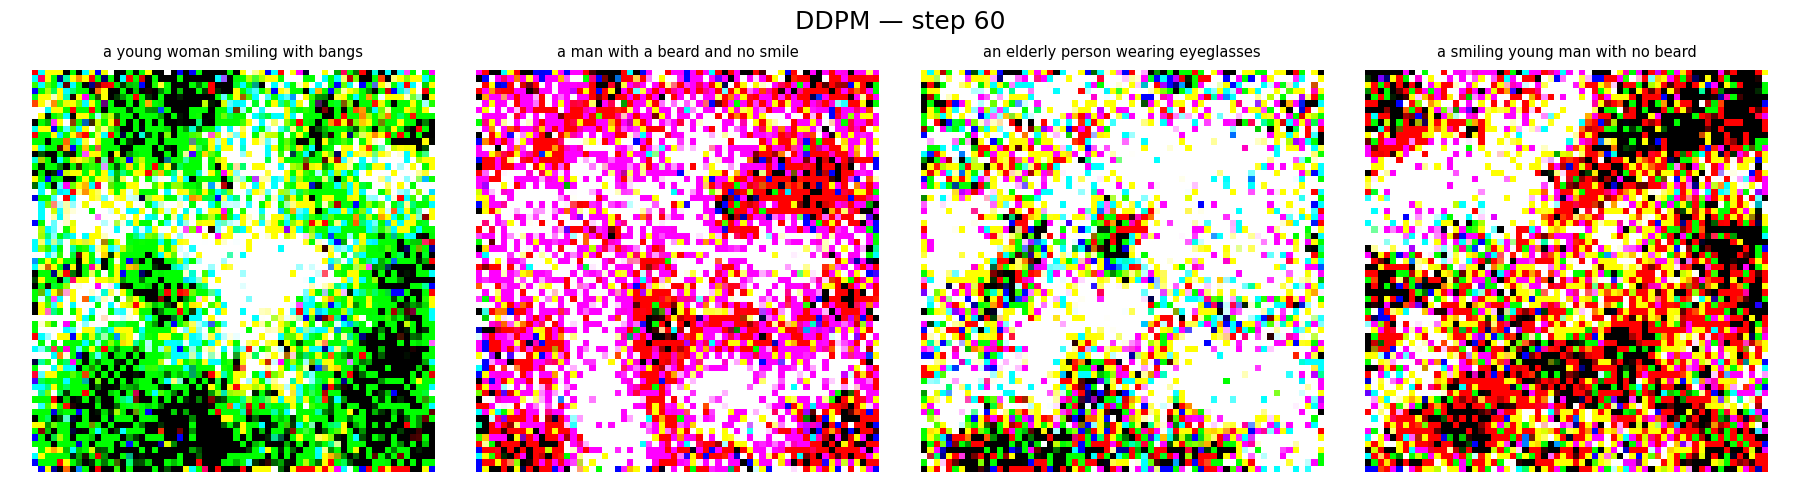
\includegraphics[width=0.85\textwidth]{figures/early_training_preview.png}
\caption{Exemple de grille de preview générée automatiquement pendant l'entraînement (ici après
seulement 60 pas d'optimisation, à titre d'illustration du mécanisme de suivi — le modèle n'a pas
encore convergé et ne produit que du bruit structuré ; un entraînement complet de plusieurs epochs est
nécessaire pour obtenir des visages reconnaissables).}
\label{fig:early-preview}
\end{figure}

\section{Interface de génération}

Un frontend web (React + Vite) et une API FastAPI permettent de générer des images depuis un
navigateur, en choisissant l'approche (DDPM ou Flow Matching), le prompt et le nombre d'étapes de
sampling. Les modèles sont chargés paresseusement par l'API (au premier appel), ce qui permet de
démarrer le serveur sans qu'aucun modèle ne soit encore entraîné.

\chapter*{Conclusion et pistes d'approfondissement}
\addcontentsline{toc}{chapter}{Conclusion et pistes d'approfondissement}

Ce document a présenté les deux grandes approches actuelles de génération d'images par transport
continu de distribution — diffusion et flow matching — depuis leurs fondements mathématiques jusqu'à
une implémentation complète et fonctionnelle. Les deux méthodes partagent bien plus qu'il n'y paraît
au premier abord : la même intuition (remplacer un grand saut génératif par une longue séquence de
petits pas), la même architecture de réseau, et ne diffèrent fondamentalement que par la façon dont le
chemin entre bruit et donnée est construit (stochastique et non-linéaire pour le DDPM, déterministe et
linéaire pour le flow matching).

\paragraph{Pistes d'approfondissement.} Plusieurs directions naturelles prolongent ce travail :
\begin{itemize}
    \item \textbf{Diffusion latente.} Remplacer la diffusion pixel-space par une diffusion dans
    l'espace latent d'un VAE (comme Stable Diffusion), pour viser une résolution supérieure à
    ressources de calcul égales.
    \item \textbf{Schémas d'échantillonnage accélérés} pour le DDPM (DDIM, solveurs d'ordre supérieur),
    qui réduisent le nombre d'étapes de génération sans réentraîner le réseau.
    \item \textbf{Fine-tuning de poids pré-entraînés} : charger des poids issus d'un modèle de
    diffusion existant dans l'architecture U-Net de ce projet, plutôt que d'entraîner entièrement
    \emph{from scratch}.
    \item \textbf{Évaluation quantitative} (FID, CLIP-score) pour comparer objectivement les deux
    approches au-delà de l'inspection visuelle.
\end{itemize}

\begin{thebibliography}{9}

\bibitem{ho2020ddpm}
J. Ho, A. Jain, P. Abbeel.
\textit{Denoising Diffusion Probabilistic Models}.
NeurIPS, 2020.

\bibitem{ho2022cfg}
J. Ho, T. Salimans.
\textit{Classifier-Free Diffusion Guidance}.
NeurIPS Workshop on Deep Generative Models, 2022.

\bibitem{lipman2023flow}
Y. Lipman, R. T. Q. Chen, H. Ben-Hamu, M. Nickel, M. Le.
\textit{Flow Matching for Generative Modeling}.
ICLR, 2023.

\bibitem{radford2021clip}
A. Radford, J. W. Kim, C. Hallacy, et al.
\textit{Learning Transferable Visual Models From Natural Language Supervision (CLIP)}.
ICML, 2021.

\bibitem{jiang2021celebadialog}
Y. Jiang, Z. Huang, X. Pan, C. C. Loy, Z. Liu.
\textit{Talk-to-Edit: Fine-Grained Facial Editing via Dialog}.
ICCV, 2021.

\bibitem{rombach2022ldm}
R. Rombach, A. Blattmann, D. Lorenz, P. Esser, B. Ommer.
\textit{High-Resolution Image Synthesis with Latent Diffusion Models}.
CVPR, 2022.

\bibitem{ronneberger2015unet}
O. Ronneberger, P. Fischer, T. Brox.
\textit{U-Net: Convolutional Networks for Biomedical Image Segmentation}.
MICCAI, 2015.

\bibitem{vaswani2017attention}
A. Vaswani, N. Shazeer, N. Parmar, et al.
\textit{Attention Is All You Need}.
NeurIPS, 2017.

\end{thebibliography}


\end{document}
